\section{resultados y discusión}

% ---------------------------------------------------------
%                       UN QUBIT
% ---------------------------------------------------------
\subsection{Relejación, excitación y desfasaje de un qubit acoplado al entorno} \label{sec: one_qubit}

% Relajación
Se considera un qubit (\textit{quantum bit}) como un sistema de dos niveles cuyo hamiltoniano es

\begin{equation} \label{eq: h_qubit}
    \mathcal{H} = \frac{\hbar}{2} \omega_q \sigma_z
\end{equation}

\noindent donde \(\omega_q\) es la frecuencia de resonancia del qubit, es decir la diferencia de energía entre los dos niveles, y \(\sigma_z\) es la matriz de Pauli.

Los autoestados correspondientes al hamiltoniano son \(|0\rangle\) y \(|1\rangle\), con energías \(\pm \hbar \omega_q / 2\). Si se prepara el sistema en uno de estos autoestados le ecuación de Schrödinger agrega solo una fase temporal a la función de onda, pero no permite transiciones. Sin embargo, se sabe que un sistema de 2 niveles acoplado a un entorno tienden a producirse efectos de relajación. Por ejemplo, si se prepara el sistema en el estado \(|1\rangle\), el sistema tiende a relajarse al estado de menor energía \(|0\rangle\). Este proceso se conoce como relajación, y se suele modelar como un operador de colapso \(C_\downarrow = \sqrt{\Gamma_\downarrow} \sigma_-\), donde \(\Gamma_\downarrow\) es la tasa de relajación y \(\sigma_-\) es el operador de aniquilación. 

Reemplazando este operador en la ecuación de Lindblad \ref{eq: Lindblad}, se tiene un sistema de ecuaciones diferenciales acopladas que describen la evolución temporal del sistema dadas por

\begin{align}
    \dot{\rho_{00}}(t) &= -\Gamma_\downarrow \rho_{00}(t), \label{eq: p00_relajacion_dif} \\
    \dot{\rho_{01}}(t) &= -i \omega_q \rho_{01}(t) - \frac{\Gamma_\downarrow}{2} \rho_{01}(t), \label{eq: p01_relajacion_dif}
    % \\
    % \dot{\rho_{10}}(t) &= i \omega_q \rho_{10}(t) - \frac{\Gamma_\downarrow}{2} \rho_{10}(t) \nonumber \\
    % \dot{\rho_{11}}(t) &= \Gamma_\downarrow \rho_{00}(t) = \Gamma_\downarrow (1 - \rho_{00}(t)) \nonumber
\end{align}

\noindent donde \(\rho_{ij}(t)\) es el elemento de la matriz densidad \(\rho(t)\) correspondiente al estado \(|i\rangle\langle j|\). Notar que se utilizó que la matriz de densidad es hermínita y de traza unitaria, por lo tanto \(\rho_{10}(t) = \rho_{01}^*(t)\) y \(\rho_{11}(t) = 1 - \rho_{00}(t)\). La solución de las ecuaciones diferenciales \ref{eq: p00_relajacion_dif} y \ref{eq: p01_relajacion_dif} es

\begin{align}
    \rho_{00}(t) &= \rho_{00}(0) e^{-\Gamma_\downarrow t} \label{eq: p00_relajacion_sol}, \\
    \rho_{01}(t) &= \rho_{01}(0)e^{- \Gamma_\downarrow t / 2} e^{-i \omega_q t}   \label{eq: p01_relajacion_sol}.
\end{align}

Notar que la relajación no solo cambia las poblaciones, sino que también disminuye las coherencias de manera exponencial. Para ilustrar este fenómeno, se simuló la evolución temporal de la población y coherencia de un qubit acoplado a un entorno, inicialmente en el estado \(|x\uparrow\rangle = \frac{1}{\sqrt{2}}(|0\rangle + |1\rangle)\), con una tasa de relajación \(\Gamma_\downarrow = 0.1\). Se asumió \(\hbar = 1\), \(\omega_q = 1\) y normalizado por \(2\pi\), de modo que el hamiltoniano se expresa en función de las frecuencias en \si{\giga\hertz}. La simulación se realizó durante un intervalo de tiempo entre \SIrange{0}{30}{\nano\second} con un paso temporal de \SI{0.001}{\nano\second}, lo que introduce un error de \(\mathcal{O}(10^{-12})\). Además, dado que la spolución de las ecuaciones no muestran cambios bruscos en las soluciones, es de esperar que el método RK4 represente de forma adecuada la solución. Estos parámetros se mantienen para todas las simulaciones posteriores de la sección. La Figura \ref{fig: x_plus_relaxation} muestra la evolución temporal de la población y coherencia del qubit.

\begin{figure} [htbp]
    \centering
    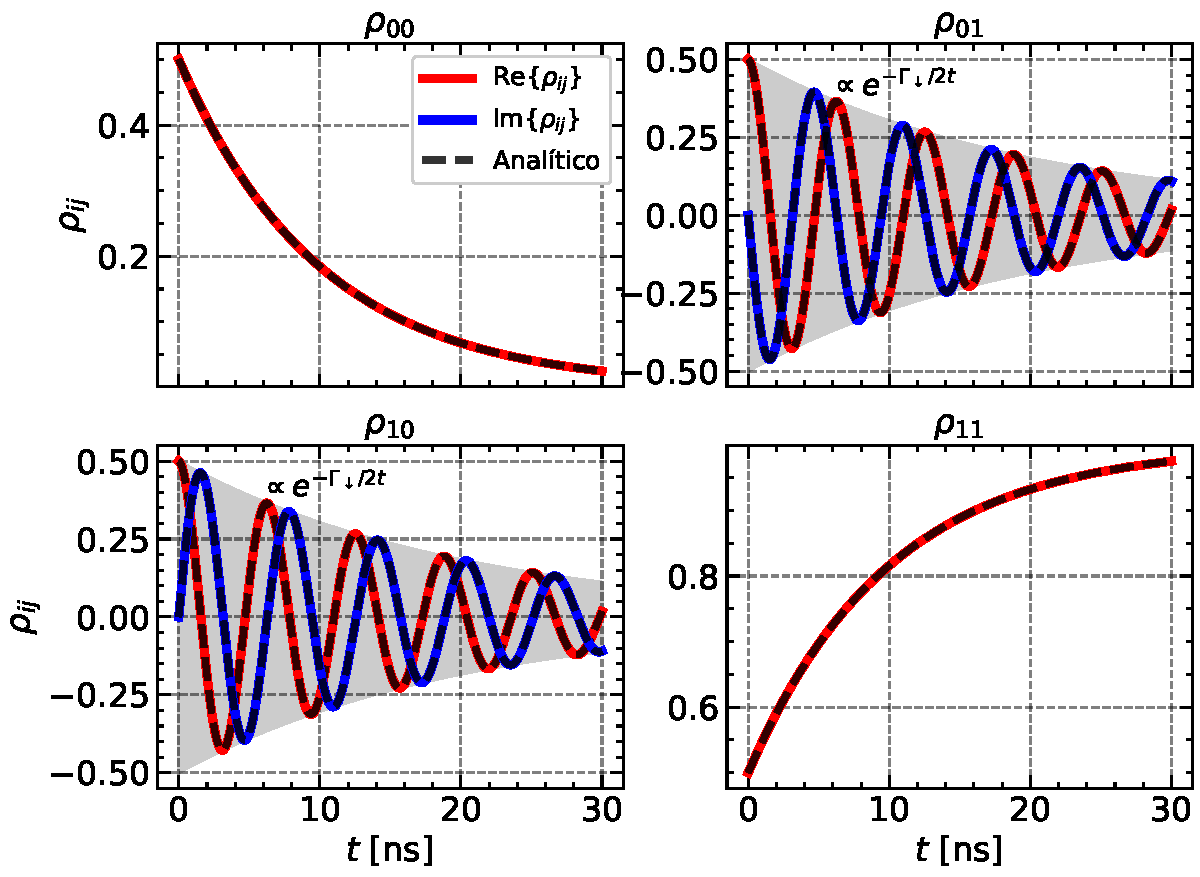
\includegraphics[width=0.5\textwidth]{figures/x_plus_relaxation.pdf}
    \caption{evolución temporal de la población y coherencia de un qubit acoplado a un entorno en el estado \(|x\uparrow\rangle = \frac{1}{\sqrt{2}}(|0\rangle + |1\rangle)\), con una tasa de relajación \(\Gamma_\downarrow = 0.1\).}
    \label{fig: x_plus_relaxation}
\end{figure}

%  Relajación + Excitación
Además de la relajación, un qubit acoplado a un entorno también puede ser excitado. Por ejemplo, si se supone que el baño térmico está formado por un conjunto de osciladores armónicos, se pueden producir transiciones entre los niveles del qubit y los niveles del baño, resultado en una excitación efectiva del sistema. Este proceso se modela como un operador de colapso \(C_\uparrow = \sqrt{\Gamma_\uparrow} \sigma_+\), donde \(\Gamma_\uparrow\) es la tasa de excitación y \(\sigma_+\) es el operador de creación. Agregando este operador junto al proceso de relacación en la ecuación de Lindblad (Ecuación \ref{eq: Lindblad}), se tiene un sistema de ecuaciones diferenciales acopladas que describen la evolución temporal del sistema dadas por

\begin{align}
    \dot{\rho_{00}}(t) &= -\Gamma_\downarrow \rho_{00}(t) + \Gamma_\uparrow \rho_{11}(t), \label{eq: p00_relajacion_excitacion_dif} \\
    \dot{\rho_{01}}(t) &= -\left[i \omega_q + \frac{1}{2}\Gamma_1 \right] \rho_{01}(t), \label{eq: p01_relajacion_excitacion_dif}
    % \\
    % \dot{\rho_{10}}(t) &= i \omega_q \rho_{10}(t) - \frac{\Gamma_\downarrow}{2} \rho_{10}(t) - \frac{\Gamma_\uparrow}{2} \rho_{10}(t) \nonumber \\
    % \dot{\rho_{11}}(t) &= \Gamma_\downarrow \rho_{00}(t) - \Gamma_\uparrow \rho_{11}(t) = \Gamma_\downarrow (1 - \rho_{00}(t)) - \Gamma_\uparrow \rho_{11}(t) \nonumber
\end{align}

\noindent donde \(\Gamma_1 = \Gamma_\uparrow + \Gamma_\downarrow\) se denomina tasa de decaimiento. Añadiendo la condición de traza unitaria, la solución de las ecuaciones diferenciales \ref{eq: p00_relajacion_excitacion_dif} y \ref{eq: p01_relajacion_excitacion_dif} es

\begin{align}
    \rho_{00}(t) &= \rho_{00}(0) e^{-\Gamma_1 t} + \frac{\Gamma_\uparrow}{\Gamma_1} \left(1 - e^{-\Gamma_1 t} \right), \label{eq: p00_relajacion_excitacion_sol} \\
    \rho_{01}(t) &= \rho_{01}(0) e^{-i \omega_q t} e^{-\Gamma_1 t / 2} \label{eq: p01_relajacion_excitacion_sol}.
\end{align}


La cantidad \(\Gamma_\uparrow/\Gamma_1\) se llama población de equilibrio, ya que representa el valor al que tiende \(\rho_{00}(t)\) cuando \(t \rightarrow \infty\). Si los procesos de relajación y excitación son iguales, la población de equilibrio es 0.5, lo que indica un estado de equilibrio térmico. 

Para ilustrar esto, se simuló la evolución temporal de la población y coherencia de un qubit acoplado a un entorno, comenzando en un estado con mayor población en el estado \(|1\rangle\) para analizar la evolución dado por \(|\psi_0\rangle = \frac{1}{\sqrt{4}} (\sqrt{3}|1\rangle + |0\rangle)\)  y con tasas de relajación y excitación iguales (\(\Gamma_\downarrow = \Gamma_\uparrow = 0.1\)). La Figura \ref{fig:3_up_relaxation_excitation} muestra los resultados de la simulación.

\begin{figure*}[htbp]
    \centering
    \subfloat[]{
        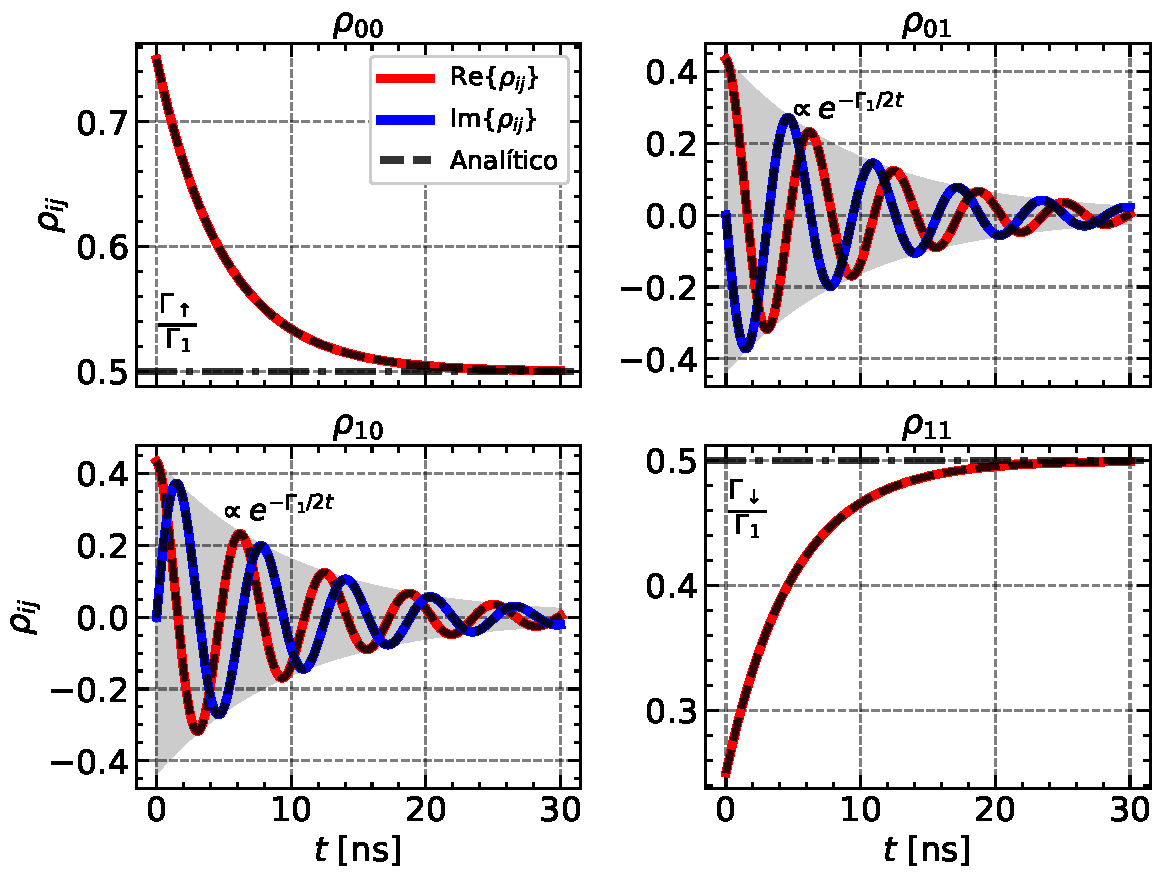
\includegraphics[width=0.48\textwidth]{figures/psi_relx_exc.pdf}
        \label{fig:3_up_relaxation_excitation}
    }
    \hfill
    \subfloat[]{
        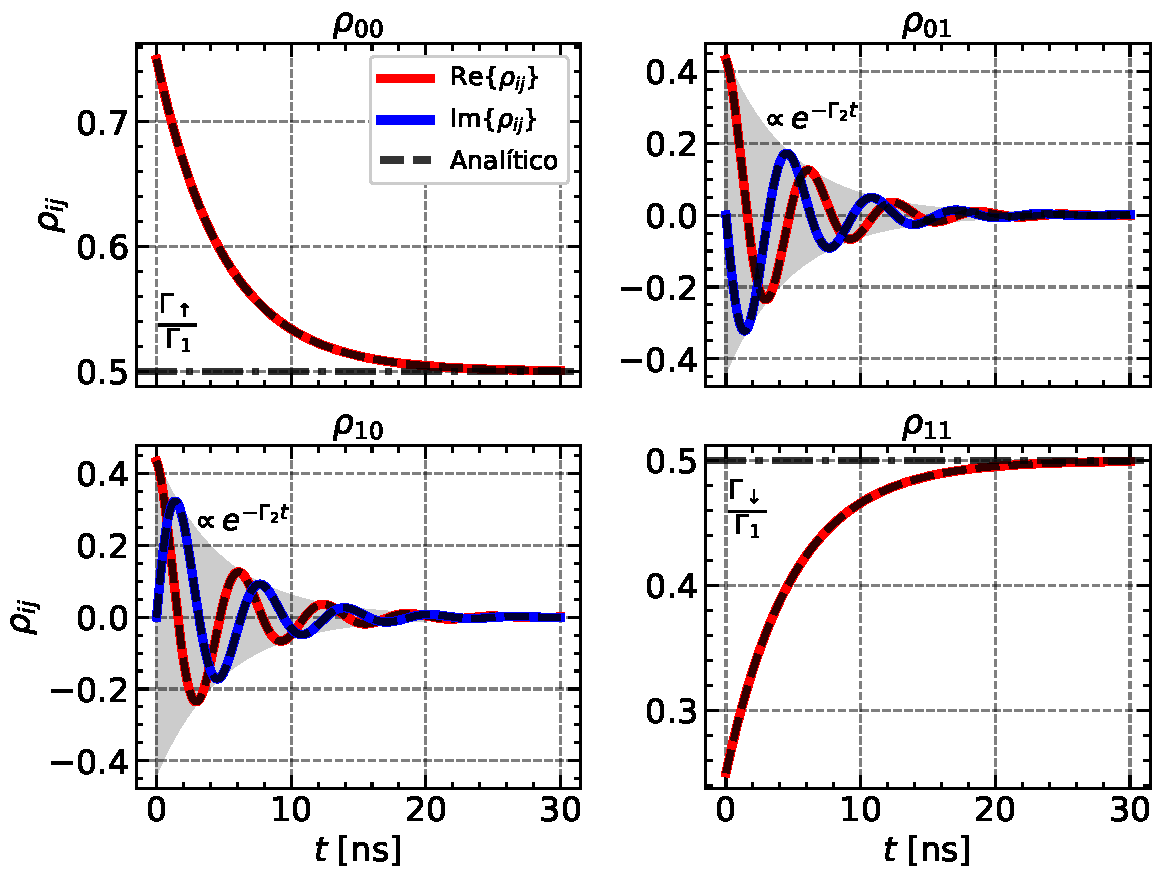
\includegraphics[width=0.48\textwidth]{figures/psi_relx_exc_desf.pdf}
        \label{fig:3_up_relaxation_excitation_dephasing}
    }
    \caption{Evolución temporal de la población y coherencia de un qubit inicialmente en el estado \(|\psi_0\rangle = \frac{1}{\sqrt{4}} (\sqrt{3}|\uparrow\rangle + |\downarrow\rangle)\), acoplado a un entorno.  
    (a) Con una tasa de relajación \(\Gamma_\downarrow = 0.1\) y una tasa de excitación \(\Gamma_\uparrow = 0.1\).  
    (b) Con las mismas tasas de relajación y excitación, y además una tasa de desfasaje \(\Gamma_\phi = 0.1\).}
    \label{fig:qubit_evolution}
\end{figure*}



% \begin{figure} [htbp]
%     \centering
%     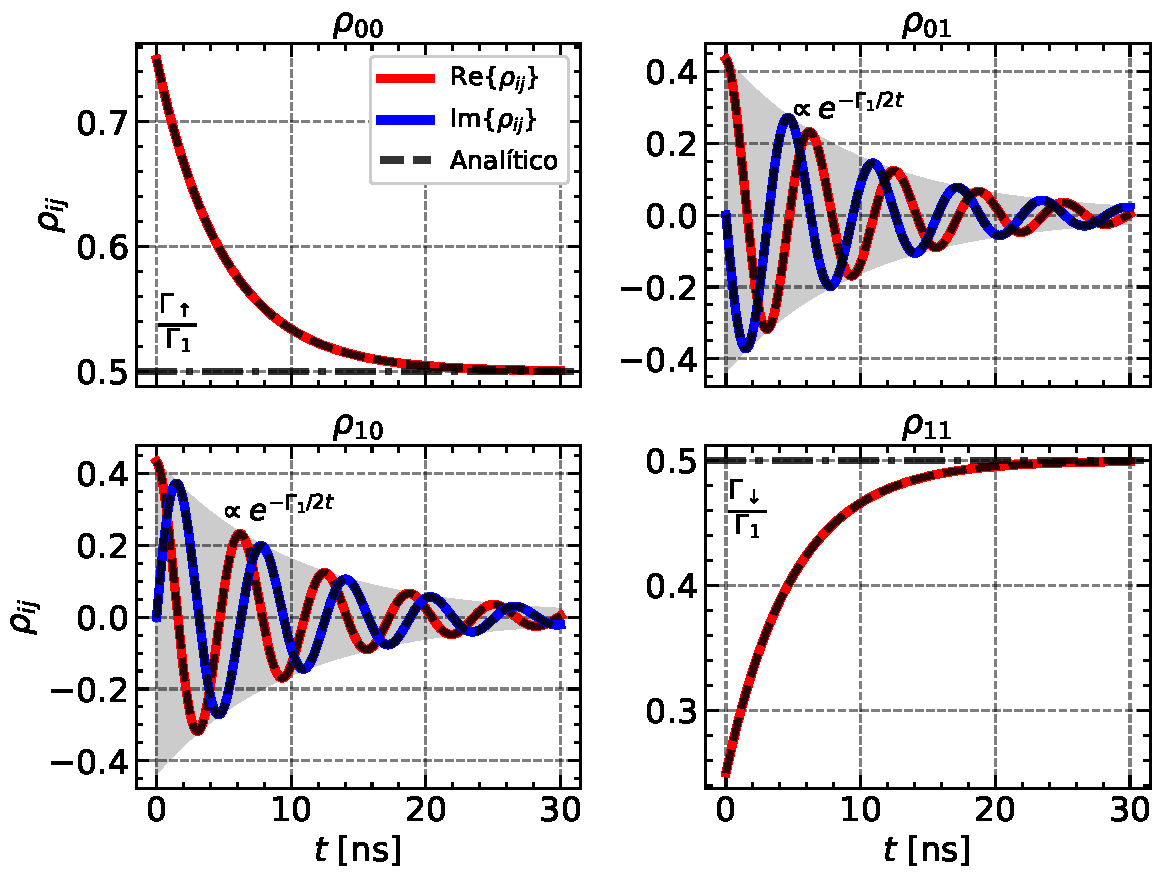
\includegraphics[width=0.5\textwidth]{figures/psi_relx_exc.pdf}
%     \caption{evolución temporal de la población y coherencia de un qubit acoplado a un entorno en el estado \(|\psi_0\rangle = \frac{1}{\sqrt{4}} (\sqrt{3}|\uparrow\rangle + |\downarrow\rangle)\), con una tasa de relajación \(\Gamma_\downarrow = 0.1\) y una tasa de excitación \(\Gamma_\uparrow = 0.1\).}
%     \label{fig: 3_up_relaxation_excitation}
% \end{figure}

Notar que las poblaciones tienden a la población de equilibrio, y que además ambos procesos disminuyen los términos de coherencia del sistema.

% Desfasaje
Por último, un qubit acoplado a un entorno también puede sufrir desfasaje, es decir modificaciones sobre los términos de coherencia. Este proceso se modela como un operador de colapso \(C_\phi = \sqrt{\Gamma_\phi/2} \sigma_z\), donde \(\Gamma_\phi\) es la tasa de desfasaje. Agregando este operador junto a los procesos de relajación y excitación en la ecuación de Lindblad (Ecuación \ref{eq: Lindblad}), se tiene un sistema de ecuaciones diferenciales acopladas que describen la evolución temporal del sistema dadas por

\begin{align}
    \dot{\rho_{00}}(t) &= -\Gamma_\downarrow \rho_{00}(t) + \Gamma_\uparrow \rho_{11}(t), \label{eq: p00_relajacion_excitacion_desfasaje_dif} \\
    \dot{\rho_{01}}(t) &= -\left(i \omega_q + \Gamma_2 \right) \rho_{01}(t), \label{eq: p01_relajacion_excitacion_desfasaje_dif}
    % \\
    % \dot{\rho_{10}}(t) &= i \omega_q \rho_{10}(t) - \frac{\Gamma_\downarrow}{2} \rho_{10}(t) - \frac{\Gamma_\uparrow}{2} \rho_{10}(t) \nonumber \\
    % \dot{\rho_{11}}(t) &= \Gamma_\downarrow \rho_{00}(t) - \Gamma_\uparrow \rho_{11}(t) = \Gamma_\downarrow (1 - \rho_{00}(t)) - \Gamma_\uparrow \rho_{11}(t) \nonumber
\end{align}

\noindent donde \(\Gamma_2 = \Gamma_\phi + \Gamma_1/2\) se denomina tasa de decoherencia. Notar que el término de desfasaje no afecta a las poblaciones, sino que solo modifica las coherencias. La solución de la Ecuación \ref{eq: p00_relajacion_excitacion_desfasaje_dif} es análoga a la ecuación \ref{eq: p00_relajacion_excitacion_sol}, mientras que la solución de la Ecuación \ref{eq: p01_relajacion_excitacion_desfasaje_dif} se obtiene reemplazando \(\Gamma_1/2\) por \(\Gamma_2\) en la ecuación \ref{eq: p01_relajacion_excitacion_sol}.

Para ilustrar esto, se simuló la evolución temporal de la población y coherencia de un qubit acoplado a un entorno, comenzando en el mismo estado que en la simulación anterior, pero añadiendo una tasa de desfasaje \(\Gamma_\phi = 0.1\). La Figura \ref{fig:3_up_relaxation_excitation_dephasing} muestra los resultados de la simulación.

% \begin{figure} [htbp]
%     \centering
%     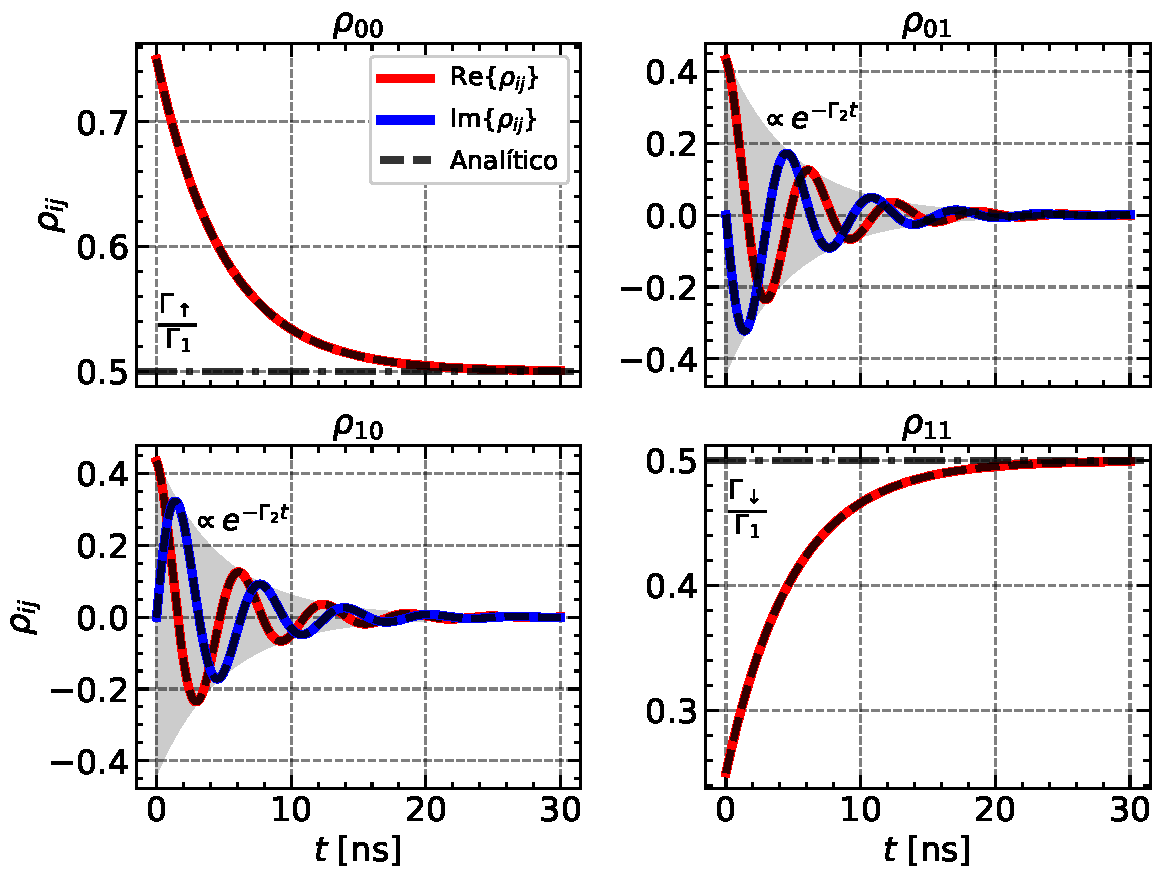
\includegraphics[width=0.5\textwidth]{figures/psi_relx_exc_desf.pdf}
%     \caption{evolución temporal de la población y coherencia de un qubit acoplado a un entorno en el estado \(|\psi_0\rangle = \frac{1}{\sqrt{4}} (\sqrt{3}|\uparrow\rangle + |\downarrow\rangle)\), con una tasa de relajación \(\Gamma_\downarrow = 0.1\), una tasa de excitación \(\Gamma_\uparrow = 0.1\) y una tasa de desfasaje \(\Gamma_\phi = 0.1\).}
%     \label{fig: 3_up_relaxation_excitation_dephasing}
% \end{figure}

Notar que en este caso, los términos de coherencia disminuyen más rápidamente debido al desfasaje. Además, la población de equilibrio se mantiene en 0.5, lo que indica que el desfasaje no afecta a las poblaciones del sistema.

% ---------------------------------------------------------
%                       DOS QUBITS
% ---------------------------------------------------------

\subsection{Entrelazamiento de dos qubit acoplados a entornos independientes idénticos} \label{sec: two_qubits}

El entrelazamiento cuántico es clave para la criptografía, la teleportación y la computación cuántica \cite{ESD,Wootters}. Aunque idealmente se espera que se mantenga el tiempo suficiente para completar tareas, en la práctica los sistemas cuánticos interactúan con entornos que lo pueden destruir el entrelazamiento. Por ello, es de intererés estudiar cómo evoluciona en el tiempo el entrelazamiento de dos qubits interactuantes con el entorno.

Se considera una situación en donde se tiene dos qubits independientes, en donde cada qubit está acoplado a un entorno en principio diferente, se tiene que el hamiltoniano total resulta

% idénticos independientes, es decir con la misma frecuencia de resonancia y sin interacción entre ellos. Además, cada qubit está acoplado a un entorno idéntico independiente, es decir con la misma tasa de decaimiento. El hamiltoniano total del sistema es

\begin{equation} \label{eq: h_two_qubits}
    \mathcal{H} = \frac{\hbar}{2} \left( \omega_q^{A} \sigma_z^{A} + \omega_q^{B}\sigma_z^{B} \right),
\end{equation}

\noindent donde \(\sigma_z^{A}\) y \(\sigma_z^{B}\) son las matrices de Pauli correspondientes a los qubits A y B, respectivamente, con frecuencias \(\omega_q^{A} = \omega_q^{B}\). Los autoestados se corresponde con el producto tensorial de los autoestados de cada qubit, es decir \(|i,j\rangle = |i\rangle^{A} \otimes |j\rangle^{B}\), con \(i,j \in \{0,1\}\). 

% Si bien \(\omega_q^{(A)} = \omega_q^{(B)}\), se escribe de esta manera para notar la simplificación de considerar qubits idénticos en cálculos posteriores. Los autoestados se corresponde con el producto tensorial de los autoestados de cada qubit, es decir \(|i,j\rangle = |i\rangle^{(A)} \otimes |j\rangle^{(B)}\), con \(i,j \in \{0,1\}\). 

Se considera solo procesos de desfasaje en los qubit, como se describe en el trabajo de Yu y Eberly (2006) \cite{ESD}, por lo que en el formalismo de Lindbland se puede modelar como un operador de colapso \(C_\phi = \sqrt{\Gamma_\phi^{A}} \sigma_z^{A} + \sqrt{\Gamma_\phi^{B}} \sigma_z^{B}\). 

% Notar que en la base de autoestados obtenidas mediante el producto tensorial, se puede escribir el Hamiltoniano y el operador de colapso en forma matricial considerando matrices de \(4 \times 4\) con índices \(i,j \in \{1, 2, 3, 4\}\) como

% \begin{equation}
%     \mathbf{e} = 
%     \begin{cases}
%         1 & \text{si } i = j = 1 \\
%         -1 & \text{si } i = j = 4 \\
%         0 & \text{en otro caso}
%     \end{cases}
% \end{equation}

% \begin{equation}
%     \mathbf{m} = 
%     \begin{cases}
%         1 & \text{si } i = j = 2 \\
%         -1 & \text{si } i = j = 3 \\
%         0 & \text{en otro caso}
%     \end{cases}
% \end{equation}



% \begin{equation}
%     \mathcal{H}/\hbar = \frac{\omega_q^{(A)}+\omega_q^{(b)}}{2} \mathbf{e} + \frac{\omega_q^{(A)}-\omega_q^{(b)}}{2} \mathbf{m}, \label{eq: h_two_qubits_matrix} \\
% \end{equation}

En la base de autoestados obtenida mediante el producto tensorial, el Hamiltoniano y el operador de colapso pueden representarse matricialmente usando matrices de \(4 \times 4\) con índices \(i, j \in \{1, 2, 3, 4\}\) como

\begin{equation} \nonumber
    \mathbf{e} =
    \begin{cases}
        1, & \text{si } i = j = 1, \\
        -1, & \text{si } i = j = 4, \\
        0, & \text{en otro caso,}
    \end{cases}
\end{equation}

\begin{equation} \nonumber
    \mathbf{m} =
    \begin{cases}
        1, & \text{si } i = j = 2, \\
        -1, & \text{si } i = j = 3, \\
        0, & \text{en otro caso,}
    \end{cases}
\end{equation}

\noindent de modo que el hamiltoniano y el operador de colapso se pueden escribir como

\begin{align}
    \mathcal{H}/\hbar &= \frac{\omega_q^{A}+\omega_q^{B}}{2} \mathbf{e} + \frac{\omega_q^{A}-\omega_q^{B}}{2} \mathbf{m}, \label{eq: h_two_qubits_matrix} \\
    C_\phi &= \left(\sqrt{\Gamma_\phi^{A}} + \sqrt{\Gamma_\phi^{B}}\right) \mathbf{e} + \left(\sqrt{\Gamma_\phi^{A}} - \sqrt{\Gamma_\phi^{B}}\right) \mathbf{m}. \label{eq: C_phi_two_qubits_matrix}
\end{align}

Por lo tanto, si se consideran qubits indénticos y entorno idénticos, entonces se tiene que \(\omega_q^A = \omega_q^B = \omega_q\) y \(\Gamma_\phi^A = \Gamma_\phi^B =\Gamma_\phi\) y se cancelan los términos de \(\mathbf{m}\) en las ecuaciones \ref{eq: h_two_qubits_matrix} y \ref{eq: C_phi_two_qubits_matrix}, lo que simplifca el cálculo de la ecuación de Lindblad. Como resultado, se obtiene un sistema de ecuaciones diferenciales acopladas que describen la evolución temporal del sistema dadas por

\begin{align}
    \dot{\rho_{ij}}(t) &= - \left(\frac{i}{\hbar} \omega_q + 2 \Gamma_\phi\right) \rho_{ij}(t) \nonumber \\
    \dot{\rho_{14}}(t) &= -2 \left(\frac{i}{\hbar} \omega_q + 2 \Gamma_\phi\right) \rho_{14}(t) \nonumber 
\end{align}

\noindent donde \(i \in \{1, 2\} \) y \(j \in \{2, 3, 4\}\) tal que \(i\neq j\) y excluyendo el caso \(i = 1, j = 4\). Notar que los elementos diagonales de la matriz densidad no se ven afectados por el desfasaje, y la simplificación de considerar qubits idénticos y entornos idénticos permite que los términos \(\rho_{23}\) y \(\rho_{32}\) no se modifiquen en la evolución temporal.

Como resultado de estas expresiones, se obtienen decaimientos exponenciales con alguna fase compleja, similar a lo que se obtuvo para el caso de un qubit, es decir

\begin{align}
    \rho_{ij}(t) &= \rho_{ij}(0) e^{-i \omega_q t} e^{-2\Gamma_\phi t} \label{sol: pij}, \\
    \rho_{14}(t) &= \rho_{14}(0) e^{-i \omega_q t} e^{-4\Gamma_\phi t} \label{eq: sol_p14},
\end{align}

\noindent con las mismas restricciones para lo índices que el caso anterior.

% Definición de concurrencia
Dado que las ecuaciones \ref{sol: pij} y \ref{eq: sol_p14} muestran que los elementos de matriz decrecen exponencialmente, es razonable que si se parte de un estado entrelazado o una combinación de estados de Bell, luego de un cierto tiempo este estado se deteriore. Para cuantificar el entrelazameinto entre dos qubit en la base acoplada, se utiliza la concurrencia definida por Woottters \cite{Wootters} dada por

\begin{equation}
    C(\rho) = \max \left\{0,\sqrt{\lambda_1}-\sqrt{\lambda_2}-\sqrt{\lambda_3}-\sqrt{\lambda_4}\right\},
\end{equation}


\noindent donde se tiene que \(\lambda_i\) son los autovalores de \(\rho(\sigma_y^A \otimes \sigma_y^B) \rho^\dagger (\sigma_y^A \otimes \sigma_y^B)\) ordenados de mayor a menor. La concurrencia es 0 si el estado es separable, y 1 si el estado es máximamente entrelazado como los estados de Bell.

Para analizar los efectos de entrelazamiento del sistema acoplado al entorno, se analizan las matrices de densidad con la forma ``estandar'' dada por

\begin{equation} \label{eq: rho_standar}
    \rho = \begin{pmatrix}
        a & 0 & 0 & w(t) \\
        0 & b & z(t) & 0 \\
        0 & z^*(t) & c & 0 \\
        w^*(t) & 0 & 0 & d
    \end{pmatrix}
\end{equation}

\noindent donde \(a,b,c,d \in \mathbb{R}\) y \(w,z \in \mathbb{C}\) con \(a+b+c+d = 1\). Este tipo de matriz se encuentra presente en una gran cantidad de situaciones físicas. Además, esta matriz incluye los estados de Bell, que son los estados máximamente entrelazados y los estados de Werner \cite{ESD}. Además, en el trabajo de Yu y Eberly (2006) \cite{ESD} se demostró que existen condiciones en las cuales se produce la muerte súbita del entrelazamiento (ESD). Para verificar estas condiciones, se tiene que analizar los casos en que la concurrencia de como resultado 0 para tiempo finito. Para esta matriz de densidad, los autovalores \(\lambda_i\) son

\begin{align}
    \lambda_{1, 2} &= \left(\sqrt{ad} \pm |w|\right)^2, \label{eq: eigval_12} \\
    \lambda_{3, 4} &= \left(\sqrt{bc} \pm |z|\right)^2 \label{eq: eigval_34}.
\end{align}

A partir de estos autovalores, se puede obtener la concurrencia como

\begin{equation}    \label{eq: concurrencia_two_qubits}
    C(\rho) = 2 \max \left\{0, |w(t)| - \sqrt{bc}, |z(t)| - \sqrt{ad}\right\},
\end{equation}

\noindent donde se consideran los casos en que \(\lambda_1\) o \(\lambda_3\) son los autovalores más grandes.

Para que se produzca ESD, se tienen que satisfacer simultaneamente las condiciones \cite{ESD}

\begin{align}
    |w(t)| - \sqrt{bc} &\leq 0, \label{eq: condicion_1_ESB_0} \\
    |z(t)| - \sqrt{ad} &\leq 0. \label{eq: condicion_2_ESB_0}
\end{align}

Notar que, según las ecuaciones \ref{sol: pij} y \ref{eq: sol_p14}, los estados de Bell \(|B_{10}\rangle, |B_{11}\rangle = \frac{1}{\sqrt{2}} (|01\rangle \pm |10\rangle)\) no se ven afectados por el desfasaje, por lo tanto la concurrencia no se modifica en el tiempo. Por otro lado, los estados \(|B_{00}\rangle, |B_{01}\rangle = \frac{1}{\sqrt{2}} (|00\rangle \pm |11\rangle)\) se ven afectados por el desfasaje, por lo que la concurrencia disminuye en el tiempo. Para estos últimos, se tiene que \(b = c = z = 0\). Según la condición \ref{eq: condicion_1_ESB_0}, para que la concurrencia sea 0 se tiene que cumplir que \(|w(t)| \leq 0\). Sin embargo, según la Ecuación \ref{eq: sol_p14}, se tiene que \(|w| = |\rho_{14}| = \rho_{14}(0) e^{-8 \Gamma_\phi t}\), la cual tiende a 0 para \(t \rightarrow \infty\). Por lo tanto, se concluye que para qubits idénticos independientes, acoplados a baños idénticos no produce ESD si se tiene como condición inicial un estado de Bell.

% por lo tanto los autovalores \ref{eq: eigval_34} son \(\lambda_3 = \lambda_4 = 0\), y la concurrencia es

% \begin{equation}
%     C(B_{00}, B_{01}) = 2 \max \left\{0, |w(t)| \right\},
% \end{equation}


% Como consecuencia, se tiene que la concurrencia para estos estados es 0 si \(|w|^2 = 0\). Sin embargo, según la Ecuación \ref{eq: sol_p14}, se tiene que \(|w| = |\rho_{14}| = \rho_{14}(0) e^{-4 \Gamma_\phi t}\), la cual tiende a 0 para \(t \rightarrow \infty\). Por lo tanto, se concluye que para qubits idénticos independientes, acoplados a baños idénticos no produce ESD. 
\begin{figure} [htbp]
    \centering
    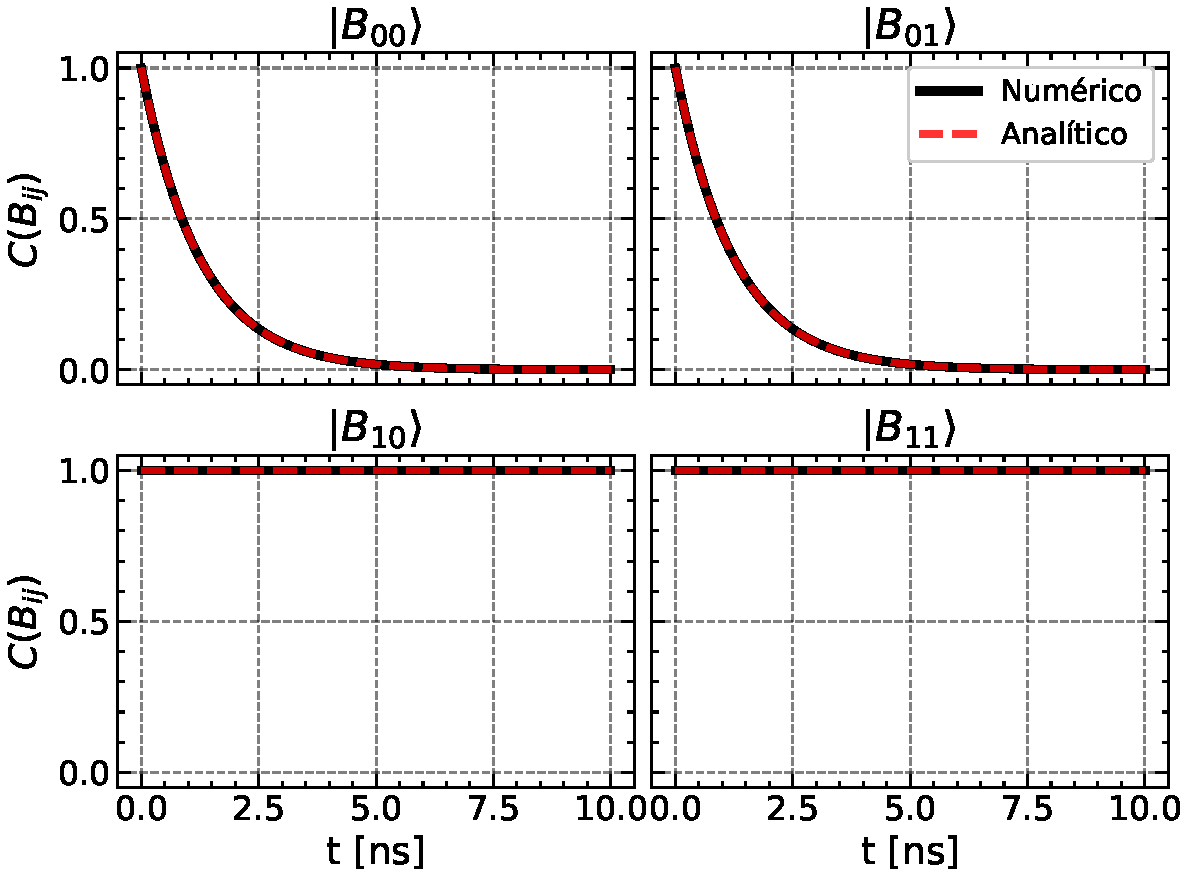
\includegraphics[width=0.5\textwidth]{figures/concurrence_bell_states.pdf}
    \caption{concurrencia para los estados de Bell obtenidos mediante resolución numérica en comparación con el resultado analítico.}
    \label{fig: concurrencia_estados_bell}
\end{figure}

Para verificar esta condición, se resolvió numericamente la ecuación de Lindbland para 2 qubits idénticos de frecuencia \SI{1}{\giga\hertz}, acoplados al entorno con un operador de colapso \(C_\phi\) con una tasa de \(\Gamma_\phi = 0.1\). Los resultados obtenidos para la concurrencia se muestra en la Figura \ref{fig: concurrencia_estados_bell}.

% \begin{figure} [htbp]
%     \centering
%     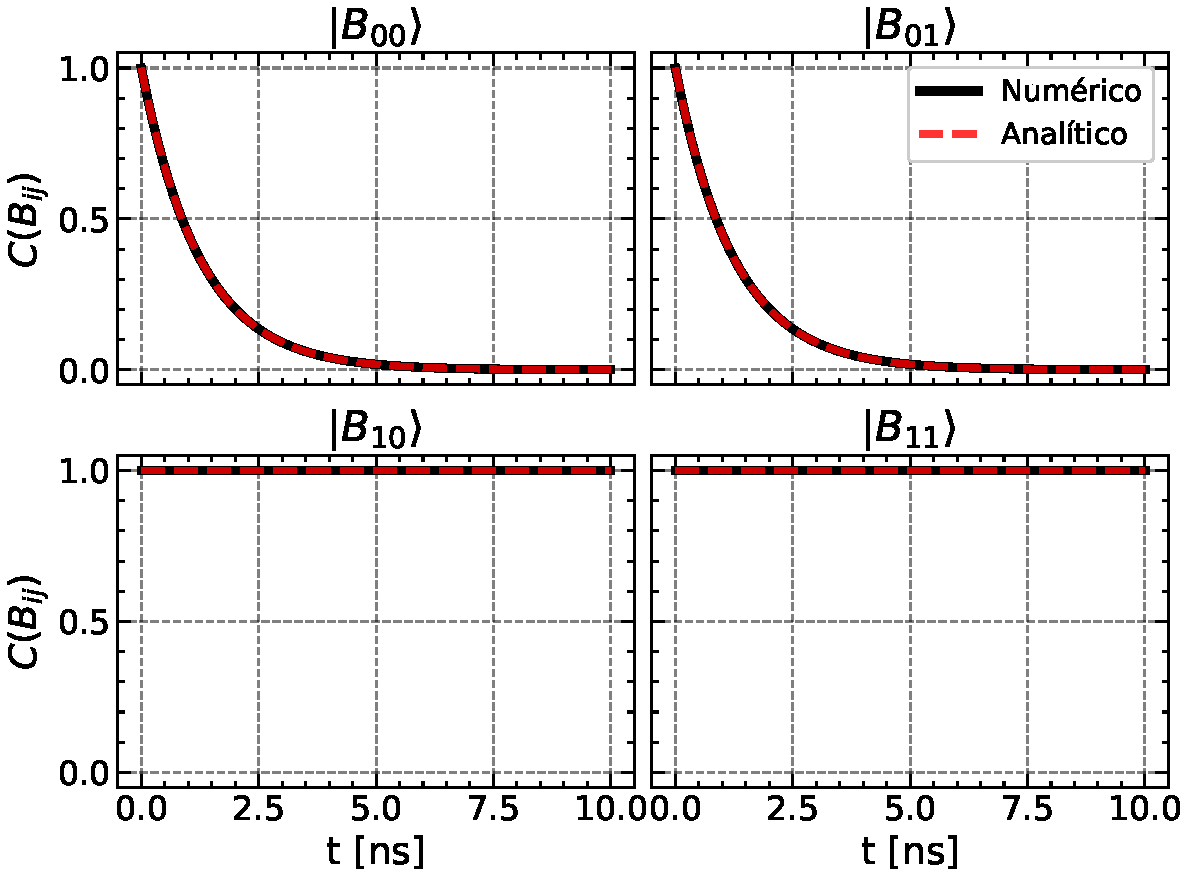
\includegraphics[width=0.5\textwidth]{figures/concurrence_bell_states.pdf}
%     \caption{concurrencia para los estados de Bell obtenidos mediante resolución numérica en comparación con el resultado analítico.}
%     \label{fig: concurrencia_estados_bell}
% \end{figure}

Luego, se seleccionaron parámetros de la matriz de la Ecuación \ref{eq: rho_standar} con valores \(a = d = 1/3\), \(b = c = 1/6\), \(w = 1/3\) y \(z = 0\), que verifica las condiciones \ref{eq: condicion_1_ESB_0} y \ref{eq: condicion_2_ESB_0}. Además, se puede obtener el tiempo en el que se produce ESD en este estado mediante la ecuación \ref{eq: sol_p14}. Como resultado, se obtiene que el tiempo en el que se produce ESD es 

% \sqrt{bc}/\rho_{03}(0)

\begin{equation} \label{eq: tiempo_ESD}
    t_d = \frac{1}{4 \Gamma_\phi} \ln \left(\frac{\rho_{03}(0)}{\sqrt{bc}}\right)
\end{equation}.

En la Figura \ref{fig: concurrencia_death_state} se muestra los resultados de la resolución numérica para la concurrencia en función del tiempo del estado mencionado, y se compara con el tiempo en el que se produce ESD según la Ecuación \ref{eq: tiempo_ESD}.

\begin{figure} [htbp]
    \centering
    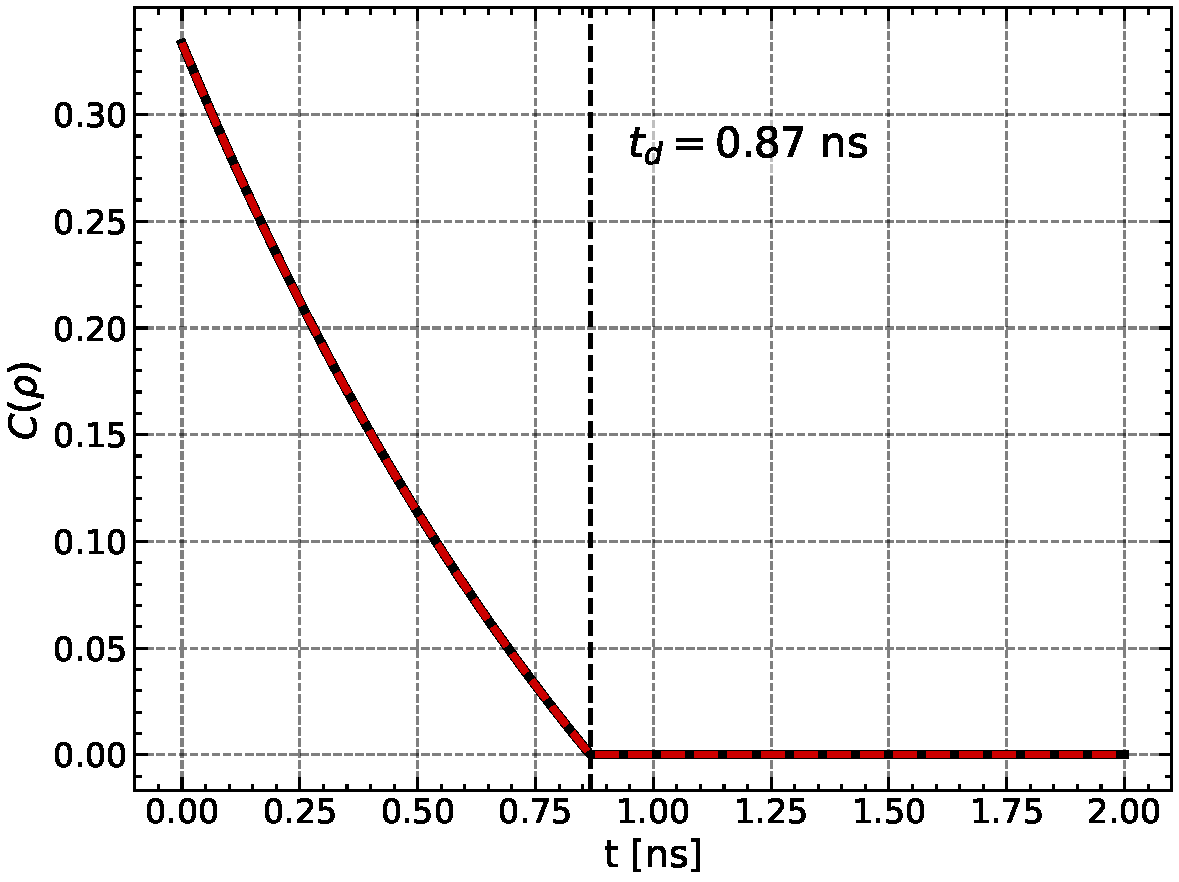
\includegraphics[width=0.5\textwidth]{figures/concurrence_death_state.pdf}
    \caption{concurrencia para un estado que verifica las condiciones de ESD en comparación con el tiempo en el que se produce ESD.}
    \label{fig: concurrencia_death_state}
\end{figure}